\documentclass{article}
\usepackage{graphicx}
\usepackage{amsmath}
\usepackage{multirow}
\usepackage[margin=1in]{geometry}

\renewcommand{\thesection}{\Roman{section}}
\renewcommand{\thesubsection}{\thesection.\Roman{subsection}}

\newcommand{\abs}[1]{\lvert #1 \rvert}

\title{TDT4171 - Assignment 4}
\author{Martin Bjerke}

\begin{document}
\maketitle

\section{Gradient Descent}

\begin{figure}[h]
  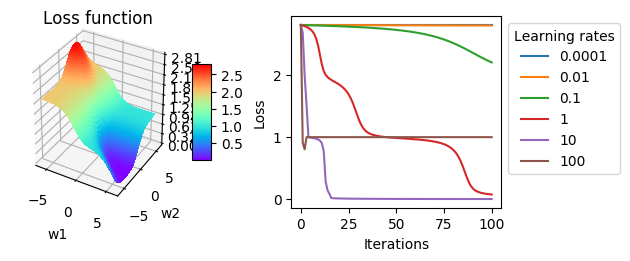
\includegraphics[scale=0.7]{plots}
  \caption{Loss function \& learningrate}
  \label{fig:plots}
\end{figure}

\begin{enumerate}
\item From  figure \ref{fig:plots} its clear that the minimum of the loss
  function(within the range of $w_i \in (6,-6)$) is $(w_1,w_2 ) = (6, -3) $.
\item Since the derivative of $\frac{\partial L_{simple}(w)}{\partial w_i}$ will
  be indifferent of $i$ I'll show the calculations of $w_i$:
  \begin{align*}
    \frac{\partial L_{simple}(w)}{\partial w_i} &= \frac{
      \left[ \sigma(w,[1,0]) -1 \right]^2 +
      \left[ \sigma(w,[0,1]) \right]^2 +
      \left[ \sigma(w,[1,1]) -1 \right]^2
      }{ \partial w_i }\\
    &=
    \frac{\left[ \sigma(w,[1,0]) -1 \right]^2}{\partial w_i} +
    \frac{\left[ \sigma(w,[0,1]) \right]^2}{\partial w_i} +
    \frac{\left[ \sigma(w,[1,1]) -1 \right]^2}{\partial w_i}\\
    &=
    \frac{1}{2} \left[ \sigma(w,[1,0]) -1 \right] \frac{\left[ \sigma(w,[1,0]) -1 \right]}{\partial w_i} +
      \frac{1}{2} \left[ \sigma(w,[0,1]) \right] \frac{\left[ \sigma(w,[0,1]) \right]}{\partial w_i} \\
    &+ \frac{1}{2} \left[ \sigma(w,[1,1]) -1 \right] \frac{\left[ \sigma(w,[1,1]) -1 \right]}{\partial w_i} \\
  \end{align*}

  Next I find the derivative of $\sigma(w, x)$:
  \begin{align*}
    \frac{\partial \sigma (w,x) }{ \partial w_i} &= \frac{ \partial (1+e^{-w^Tx} )^{ -1 }}{\partial w_i}  \\
    &= - \left( \frac{1}{1+e^{-w^Tx}} \right)^{-2} \cdot \frac{\partial ( 1+e^{-w^Tx} )}{\partial w_i} \\
    &= - \left( \frac{1}{1+e^{-w^Tx}} \right)^{-2} \cdot (-x_i e^{-w^Tx}) \\
    &= x_i \frac{e^{-w^Tx}}{1+e^{-w^Tx}} \cdot \frac{1}{1+e^{-w^Tx}} \\
    &= x_i \frac{1+e^{-w^Tx}-1}{1+e^{-w^Tx}} \cdot \frac{1}{1+e^{-w^Tx}} \\
    &= x_i \left[ \frac{1+e^{-w^Tx}}{1+e^{-w^Tx}} - \frac{1}{1+e^{-w^Tx}} \right] \cdot \frac{1}{1+e^{-w^Tx}} \\
    &= x_i \left[ 1 - \frac{1}{1+e^{-w^Tx}} \right] \cdot \frac{1}{1+e^{-w^Tx}} = x_i \sigma (w,x) \left[ 1 - \sigma (w,x) \right]
  \end{align*}
  Inserting this:
  \begin{align*}
    \frac{\partial L_{simple}(w)}{\partial w_i} &=
      \frac{x_i}{2} \left[ \sigma(w,[1,0]) -1 \right] \sigma (w,[1,0]) \left[ 1 - \sigma (w,[1,0]) \right] \\
      &+ \frac{x_i}{2} \left[ \sigma(w,[0,1]) \right] \sigma (w,[0,1]) \left[ 1 - \sigma (w,[0,1]) \right] \\
      &+ \frac{x_i}{2} \left[ \sigma(w,[1,1]) -1 \right] \sigma (w,[1,1]) \left[ 1 - \sigma (w,[1,1]) \right] \\
  \end{align*}

  This derivative results in the following derivative of the loss function:
  \begin{align*}
    \nabla_wL_{simple}(w) &= \left[ \frac{\partial L_{simple}(w)}{\partial w_1},
                                \frac{\partial L_{simple}(w)}{\partial w_1} \right] \\
    \frac{\partial L_{simple}(w)}{\partial w_1} &=
      - \frac{1}{2} \left( \sigma(w,[1,0])\left[ \sigma(w,[1,0] - 1) \right]^2 +
      \sigma(w,[1,1])\left[ \sigma(w,[1,1] - 1) \right]^2 \right) \\
    \frac{\partial L_{simple}(w)}{\partial w_1} &=
      - \frac{1}{2} \left( \sigma(w,[0,1])^2\left[ \sigma(w,[0,1]) \right] +
      \sigma(w,[1,1])\left[ \sigma(w,[1,1] - 1) \right]^2 \right) \\
  \end{align*}

\item From  figure \ref{fig:plots} you can see that with a learningrate of 1 and
  10 minimizes $L_{simple}$ after 100 and 15 iterations each, while the smaller
  iterations bearly starts to minimize after 100 iterations.
\end{enumerate}

\section{Perceptron}
\begin{enumerate}
\item Continuing the calculations from above:
  \begin{align*}
    \frac{\partial L_n(w,x_n,y_n)}{\partial w_i} =
    x_i \cdot \left[ \sigma(w,x_n) - y_n \right] \left[ 1 - \sigma(w,x_n) \right] \sigma(w,x_n)
  \end{align*}

\item The table below show the avgarge when the perceptron was trained 10 times
  with 200 iterations, time is given in seconds and errors are given in percent
  where 0\% meaning everything was classified correctly. \\
  \begin{tabular}{|c|c|c|c|c|}
    \hline
    \multirow{2}{*}{Data set} & \multicolumn{2}{|c|}{Batch} &  \multicolumn{2}{|c|}{Stochastic} \\
    \cline{2-5}
    & Training time(s) & Avg. error(\%) & Training time(s) & Avg. error(\%) \\
    \hline
    Big\_nonsep   & 57.86 & 19.3 & 0.01 & 21.4 \\
    \hline
    Big\_sep      & 59.31 & 00.9 & 0.02 & 1.5 \\
    \hline
    Small\_nonsep & 12.07 & 20.6 & 0.01 & 21.3 \\
    \hline
    Small\_sep    & 11.89 & 00.8 & 0.01 & 2.6 \\
    \hline
  \end{tabular} \\
  From the table above it is clear that batch gradient descent training is
  slower, but slightly more accurate on these data sets. This result concurces
  with the algorithm as batch gradient descent calculates $T \cdot (d) \cdot
  \abs{D_{train}}$ gradients while stochastic only calculates $T \cdot (d)$.
  By looking further on the number of gradients calculated by the methods the
  correlation between the times also becomes apparent; Stochastic doesn't depend
  on the size of the data set and calculates $200 \cdot 2 = 400$ gradients,
  while batch calculates $400 \cdot 11000$ and $400 \cdot 2200$ gradients on 200
  iterations. As the big data sets are 5 times as large as the small, the
  difference in training time correlates with this by beeing 5 times as large.
  As one would believe the non separable data sets are more inacurate and the
  seperability of the data set has no effect on the time used by the different
  methods since the code does not take this into consideration when calculating
  the gradients.

\item Training the perceptron using stochastic gradients descent on the the
  small seperatable data set and ploting the results gives the following plot. \\
  \noindent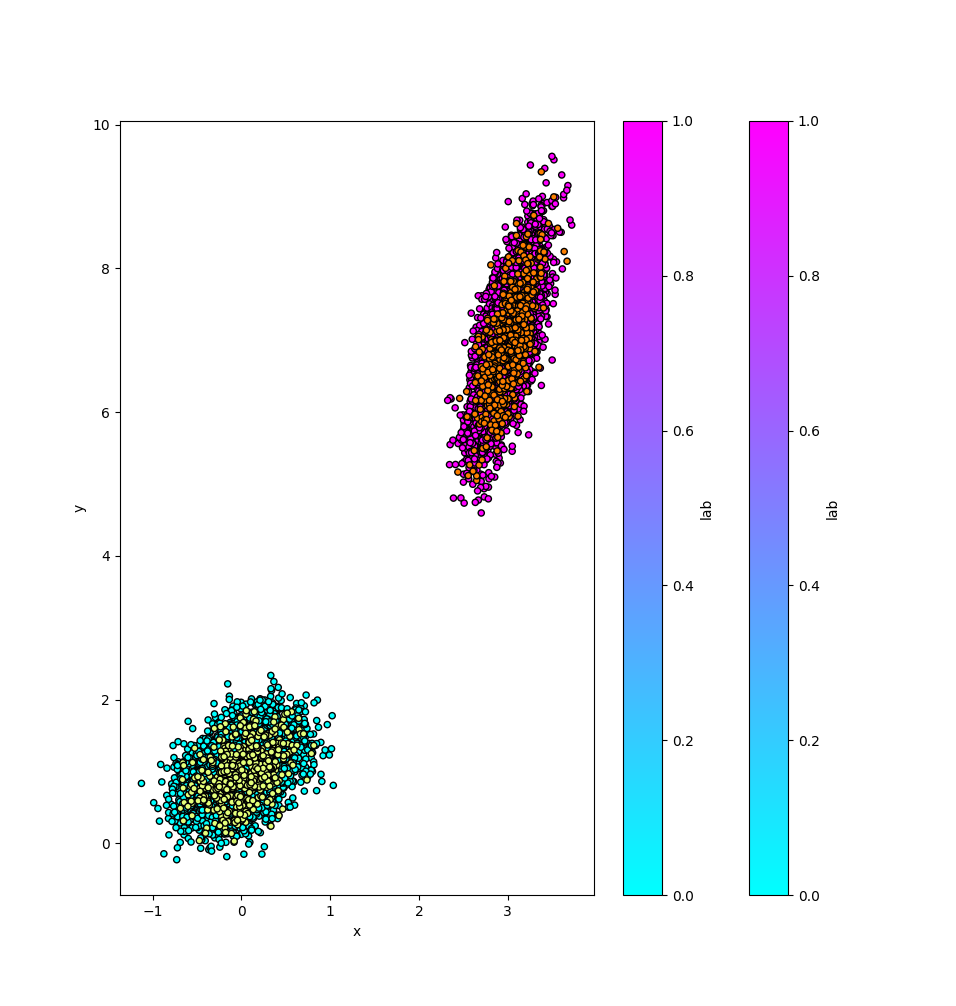
\includegraphics[scale=0.7]{plots_percep}

\item The same dataset and algorithm as above gives the following results(plots
  are placed after the discussion): \\
  \begin{tabular}{|c|c|c|}
    \hline
    Iterations & Error(\%) & Time \\
    \hline
    10 & 50.0 & 0.008 \\
    20 & 21.8 & 0.009 \\
    50 & 49.6 & 0.009 \\
    100 & 1.8 & 0.010 \\
    500 & 0.0 & 0.019 \\
  \end{tabular} \\
  The first mention should be the 49.6\% error rate on 50 iterations. The
  results are for 5 different sets of initial weights, so the error did not increase from 20 to 50
  iterations. Other then this the general trend is a decreased error rate for
  each iteration, concuring with results gotten on the previous tasks.

  \noindent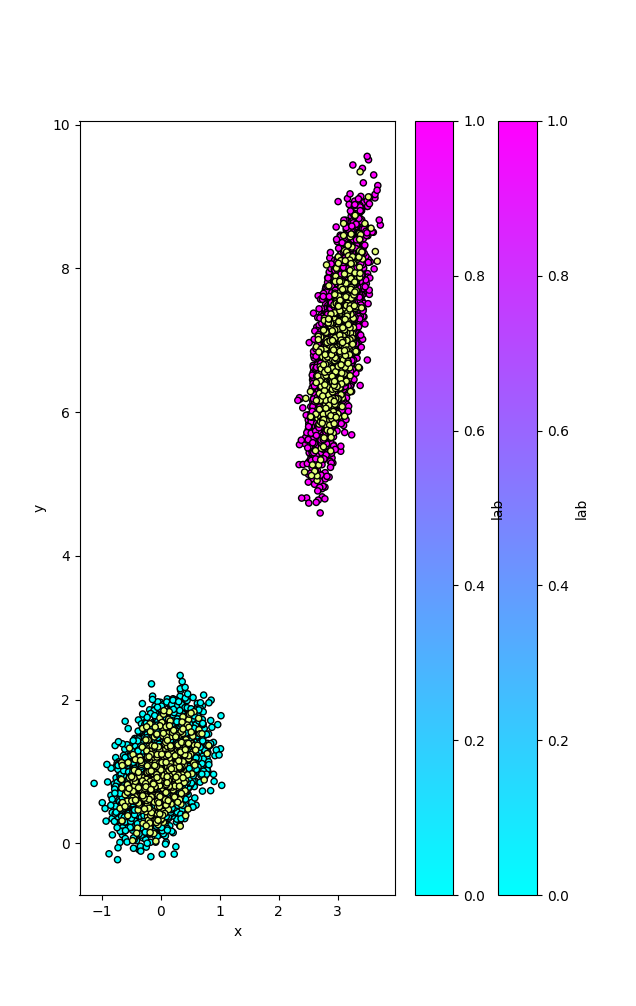
\includegraphics[scale=0.5]{plot_10}
  \noindent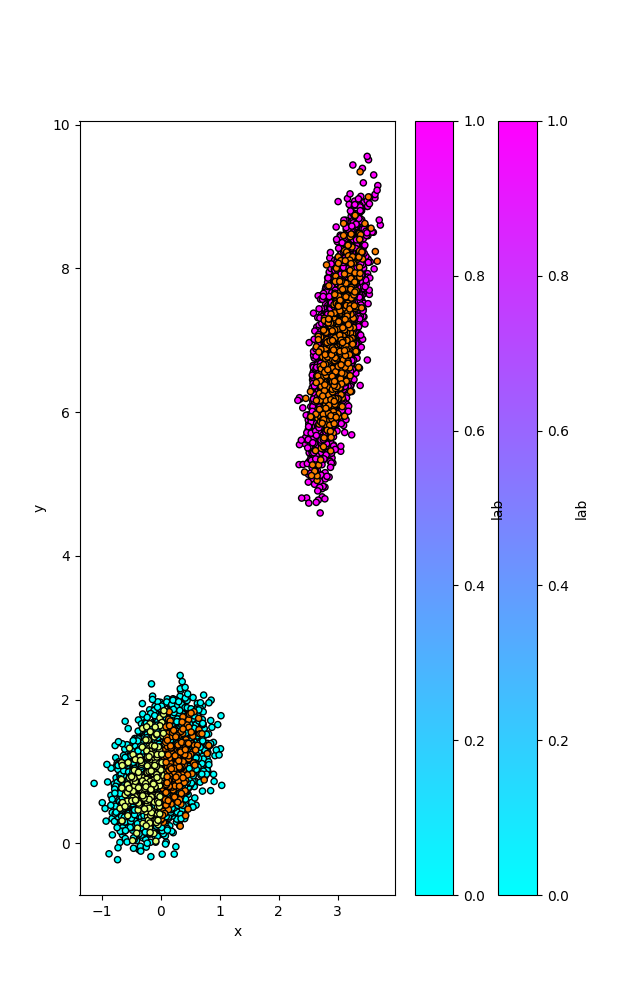
\includegraphics[scale=0.5]{plot_20}
  \noindent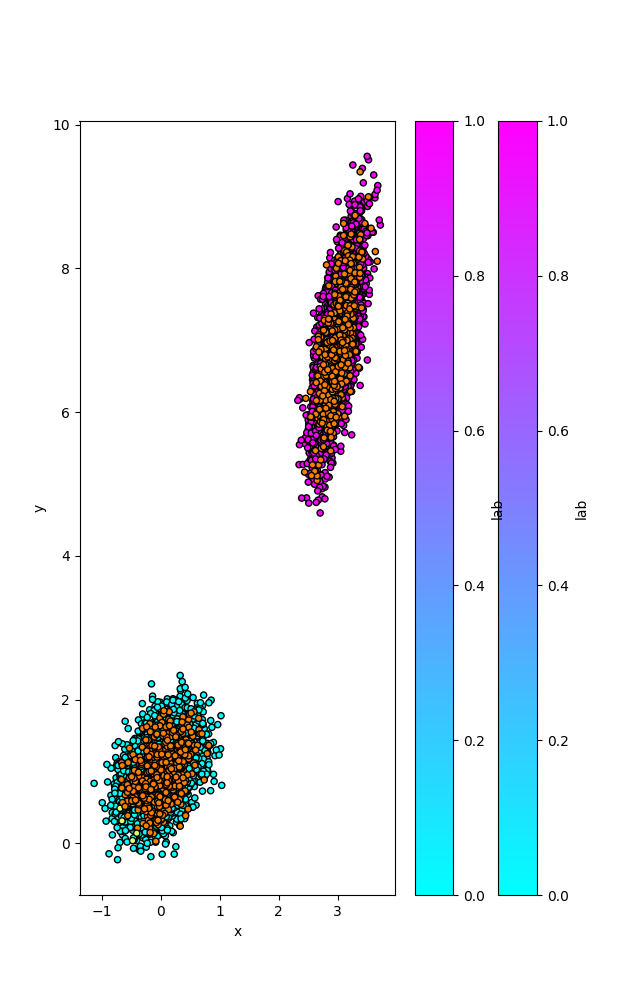
\includegraphics[scale=0.5]{plot_50}
  \noindent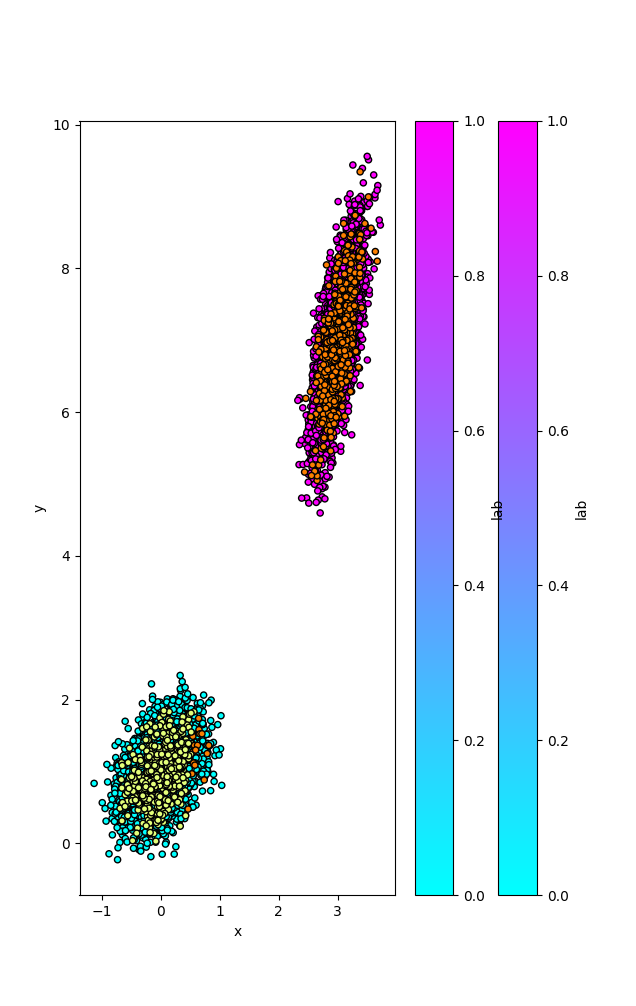
\includegraphics[scale=0.5]{plot_100}
  \noindent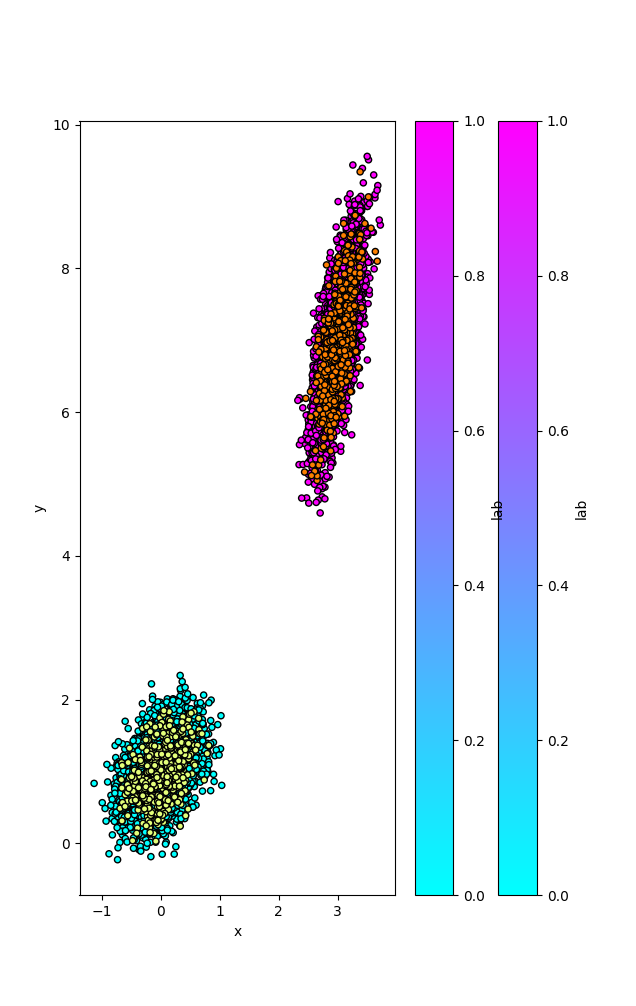
\includegraphics[scale=0.5]{plot_500}
\end{enumerate}

\end{document}
